\documentclass[12pt, a4paper, titlepage]{article}

\usepackage[top=2cm, bottom=2cm, left=2cm, right=2cm]{geometry}
\usepackage{fancyhdr}
\pagestyle{fancy}

\newcommand{\tabitem}{~~\llap{\textbullet}~~}



\usepackage{graphicx, latexsym}
\usepackage{setspace}
\usepackage{amssymb, amsmath, amsthm}
\usepackage{bm}
\usepackage{epstopdf}
\usepackage[]{hyperref}
\usepackage{xcolor}
\usepackage{apacite}
\usepackage[]{natbib}
\emergencystretch=1em
\hypersetup{
    pdftitle={Research Report},
    pdfauthor={Vera Oosterveen},
    pdfsubject={Master thesis, EMOS},
    pdfkeywords={},
    bookmarksnumbered=true,     
    bookmarksopen=true,         
    bookmarksopenlevel=1,       
    colorlinks=true,      
    colorlinks=true,
    citecolor=blue, % changes colors of links in document
    linkcolor=blue,
    urlcolor=blue,           
    pdfstartview=Fit,           
    pdfpagemode=UseOutlines,      
    pdfpagelayout=TwoPageRight
}

\graphicspath{ {./images/} }

%\singlespacing
\onehalfspacing
%\doublespacing


%%%%%%% TO DO

% Iets meer toevoeging studie, eind inleiding?

% nadenken over logloss loglikelihood

% outro 3.1

% iteration: until certain threshold

% manual checks grote bedrijven
	% The SBI codes for big, influential companies are actively checked by SN.
	% In practice, big, influential companies are manually checked at Statistics Netherlands. We can use this knowledge in our advantage, by initaiting the algorithm based on the large companies.

% EM tabel beter; en uitleggen initial values

% application to GBR

%%%%%%% varieren met verhoudingen van sets?
% percentage fouten


\begin{document}
\title{Predicting incorrect labels: combining (noisy) existing data and text classification}
\author{Vera Oosterveen \\   \multicolumn{1}{p{.7\textwidth}}{\centering\emph{Statistics Netherlands \& Utrecht University}}}
\date{\today}
\maketitle

							%%%%%%%%%%
							\begin{abstract}
							***Insert abstract :)***
							\end{abstract}
							%%%%%%%%%%


							%%%%%%%%%%
							\section{Introduction}
							\label{section:intro}
							%%%%%%%%%%

National Statistical Institutes (NSI’s) aim to produce official statistics to contribute to the public debate and policy development. Business statistics, such as statistics on turnovers and bankruptcies, give insights into different facets an economy. These business statistics are often presented by industry, groupings of enterprises with similar economic activities. A classification system for economic activities that is widely used in Europe is the NACE (Nomenclature statistique des activités économiques dans la Communauté Européenne). The NACE is a hierarchical classification and consists of four-digit codes. National Statistical Institutes (NSI’s) may introduce a fifth digit, as Statistics Netherlands did in the \textit{Standaard Bedrijfsindeling} (SBI).

The SBI codes for Dutch enterprises can be found in the general business register (GBR). An enterprise is described by Statistics Netherlands as 'statistical unit' and can be a combination of multiple legal units. When a 'legal unit' is registered at the chamber of commerce the SBI code is determined. 

However, one may question the quality of the SBI codes found in the GBR. \citet{Christensen2008} found that, considering all NACE categories, 18 percent of a sample of Danish firms with at least 5 employees were misclassified. There are no recent quality evaluations available for all NACE codes in the Netherlands. But, for the Dutch car trade sector, with 9 sub-categories, \citet{DeldenScholtusBurger} found that small enterprises (less than 10 employees) in certain sectors had a probability of 50 percent of misclassification.

The SBI codes in the GBR might be incorrect for several reasons. An incorrect code can be appointed during registration, the structure of an enterprise changes over time, or there might be changes in the activity over time. Changes in economic activity are rarely registered \citep{Christensen2008, DeldenScholtusBurger} since this is not obligatory. The correctness of the SBI codes is of great importance for the quality of the business statistics. Misclassifications in the SBI codes could lead to inaccurate, biased output statistics.

To avoid costly and time-consuming manual checks, NSI’s can use additional data sources to validate or supplement the current data sources. Previous research tried to predict the correct economic activity code using text classification approaches. Textual descriptions of the activity \citep{Caterini} or website texts \citep{Roelands, Berardi, Heidi} were deployed to automate the classification of enterprises using machine learning techniques. However, these attempts resulted in low accuracy or high misclassification rates. 

Websites are not necessarily created to describe an economic activity, but are aimed at branding, selling products or services. This has two consequences. Firstly, it complicates designing an accurate text classifier. Secondly, the observed label in the GBR might be more informative than the website text. Solely relying on text classification algorithms might not be the optimal strategy to deal with the possibly ‘noisy’ labels in the GBR.

Instead of predicting the correct label for each case, the focus in this study is on estimating which cases are labeled incorrectly. If the incorrectly labeled cases can be pointed out, these can be corrected with manual editing. 

The goal of the current research is therefore to create a method to point out the incorrectly labeled cases. To find these erroneous cases both the observed label and a predicted label, based on a machine learning algorithm, are included in the proposed method. Including two labels for every enterprise leads to the introduction of a variable that indicates whether there is an agreement between those two labels. An agreement between the two labels would lead to more trust in the labels, i.e. a lower probability of being erroneous for that enterprise.

To point out the incorrectly labeled cases, we include the probability of an error. Other studies that tried to locate erroneous cases assumed a random error-pattern \citep{Sigurdsson,Eskin,DiZio}. An average probability of being incorrect was included in the models to account for the noise. However, we believe the probability of an error might depend on characteristics of the enterprise. \citet{DeldenScholtusBurger} found that enterprise characteristics, such as size class and the number of legal units, influence the probability of an classification error. Instead of assuming a random-error pattern, the current research will account for heterogeneous error probabilities.

% For that reason, the proposed method explicitly models the probability of an error with a logistic regression model.


							%%%%%%%%%%
							\section{Related work}
							\label{section:related}
							%%%%%%%%%%

The effects of noisy labels on commonly-used algorithms (e.g. Support Vector Machines (SVMs), logistic regression, k-nearest neighbours) are well studied \citep{Pech, Nettleton}. In general, the performance of an algorithm decreases when labels in the training data are noisy. Although, some algorithms are less influenced by label noise than others \citep{Frenay}. Furtermore, we can distinguish two main approaches when dealing with label noise \citep{Frenay}: filtering approaches and  incorporating a model for the label noise within an algorithm. 

With a filtering approach, the label noise is handled in the data preprocessing stage. Labels that are suspected to be noisy are simply removed from the training set \citep{Brodley}. Removing the suspecte noisy cases from the training set possibly lead to higher classification accuracy, but filtering is problematic when training data is scarce. Also, good classifiers are needed to detect misclassified cases, and learning from noisy labels results in weak classifiers: a chicken-and-egg dilemma as pointed out by \citet{Angelova}.

Label noise robust variations of common classifiers have been proposed for, among others, logistic regression \citep{Bootkrajang, Rantalainen}), SVMs \citep{Stempfel}, and neural-networks \citep{Sigurdsson, Sukhbaatar}). Or, with a Bayesian approach, a prior on the mislabeling probabilities is included in the model (see \citet{Frenay} for references).

Some approaches for incorporating label noise in a model are interesting in particular, since these are more closely related to the current research. These approaches assume a mixture model. By imposing a mixture model, the population is assumed to consist of multiple subpopulations. A different distribution can be modeled for each subpopulation. A mixture model can be applied to deal with label noise, or to find anomalies or outliers in a dataset. \citet{DiZio, Eskin} applied such a mixture model. They assumed that the erroneous data and the error-free data came from different distributions. Detecting the noisy cases is then identical to finding out to which distribution a case belongs.

The current study has a similar motivation as the earlier studies of \citet{DiZio, Eskin}, but without assuming a specific distribution for the erroneous and error-free data. In the current research, the erroneous cases will be selected based on probability estimates, which is explained in depth in Section~\ref{section:probs}. In addition, the previous research on using website texts to predict the SBI codes will be expanded. As \citet{Nigam} showed, a classifier can be improved by when both labeled and unlabeled data are used for training. By assuming that it is unknown whether an enterprise has the correct SBI code or not, these cases are treated as unlabeled. Therefore, we propose a method where the machine learning model used to predict SBI codes will be iteratively updated by including instances in the training set that are considered correct. 

\bigskip

This paper proceeds as follows. In Section~\ref{section:method}, we describe the proposed methodology to find erroneous labeled cases. In turn, we will elaborate on the different experiments that we ran to test the method in Section~\ref{section:experiments}. Lastly, results and conclusions are given.




							%%%%%%%%%%
							\section{Methodology}
							\label{section:method}
							%%%%%%%%%%

In this research, the following aspects are combined in the proposed method:
\textcolor{red}{I don't really know how to open this section...}


\begin{enumerate}
\item The predicted label, based on an enterprises' website,
\item The observed label, as can be found in the GBR,
\item The agreement between the observed label and the predicted label,
\item The probability of an error.
\end{enumerate}

% Predicted label
The predicted label is obtained by fitting a machine learning model, the method is not restricted to a specific classifier.  The website text serves as the input for the machine learning model. URLs for websites are obtained from the GBR, or via an external party when a URL was missing in the GBR. Only the main page of each website is scraped. The text from the main page is tokenized, e.g. split into smaller parts that can serve as features. Moreover, the observed label, and the agreement between the observed label and the predicted label will be included. 

% Prob of error / Logistic regression
We assume that characteristics of an enterprise affect the probability of having an erroneous label. A logistic regression is modeled to relate characteristics of enterprises to the probability of an error. These characteristics are \textit{the size class}, \textit{the number of legal units that together form the statistical unit}, \textit{the number of different activities in the legal units}, \textit{an enterprises' age}, \textit{the SBI codes for the main and secondary economic activity of an enterprise}. These characteristics are all available in the GBR.
\bigskip

First of all, all mathematical notation will be introduced in the following paragraph. In Section~\ref{section:probs} we explain how we derive the probability of an erroneous label for each case, based on the components mentioned above. These probabilities are estimated with an EM algorithm, as explained in Section~\ref{section:em}.

							\subsection{Notation}

\textbf{The predicted label.} Let $y^*_i = k$ denote the SBI code predicted by the machine learning model for unit $i$. The input for the machine learning model are the features of the website text, denoted by $\zeta_i$. The parameters of the machine learning model are denoted by $\theta^M$. 
%Any machine learning model that gives provides predicted class probabilities would work

\textbf{The observed label.} The SBI code as found in the GBR is denoted by $\hat{y}_i = h$. 

\textbf{The agreement.} The predicted code $y^*_i = k$ and the observed code  $\hat{y}_i = h$ are compared. Let $a$ denote this agreement, with $a \in \{0,1\}$. Let $a=1$ if the two codes agree and $a=0$ otherwise.

\textbf{The probability of an error.} Finally, we introduce a latent variable, $z_i$, that represents whether a unit's observed code in the GBR is correct or erroneous. Let $z_i = 0$ if the code in the GBR is the true code and $z_i = 1$ otherwise. The variable $z_i$ can be modeled as a function of enterprise characteristics using logistic regression. The probability of an erroneous label, $P(z_i = 1)$, may depend on characteristics such as the size class or the number of legal units \citep{DeldenScholtusBurger}. Enterprise characteristics are denoted by  $u_i$. Let $\theta^R$ denote the parameters of the logistic regression model.
% introduce pi!!!
The full set of model parameters is therefore $\theta \in \{ \theta^M, \theta^R\}$. 

					%%%%%%%%%%
					\subsection{Deriving the probability of being erroneous}
					\label{section:probs}
					%%%%%%%%%%

Eventually, we are interested in the probability that a unit is incorrectly labeled, given the agreement between observed and predicted code, enterprise characteristics, features derived from the website text, and the model parameters. This is defined as $\tau_i$:

						\begin{equation} \label{eq:1}
\tau_i(\hat{a}_i = a) \equiv P(z_i = 1 | \hat{a}_i = a, \hat{y}_i = h, \zeta_i, u_i, \theta).
						\end{equation}

To find a probability for Equation~\ref{eq:1}, we use \textit{Bayes' Theorem} with multiple conditions:

						\begin{equation*} \label{eq:bayes}
P(A | B, C) =  \frac{P(A | C) P(B | A, C)}{P(A|C)P(B|A,C) + P(A^C|C)P(B|A^C, C)}   .
						\end{equation*}

Substituting elements of Equation~\ref{eq:1} into Bayes' Theorem gives: 
%A for $z_i = 1$, B for $\hat{a}_i = 1$, and C for $\hat{y}_i = h, \zeta_i, u_i, \theta$ gives:

						\begin{equation}\label{eq:2}
\tau_i(\hat{a}_i = 1) = (z_i = 1 | \hat{a}_i = 1, \hat{y} = h, \zeta_i, u_i, \theta) = 
						\end{equation}

						\begin{equation}\label{eq:3}
\frac{P(z_i = 1|\hat{y}_i = h, \zeta_i, u_i, \theta)P(\hat{a}_i=1|z_i=1, \hat{y}_i = h, \zeta_i, u_i, \theta) }
{\sum_{z=0,1}P(z_i=z|\hat{y}_i = h, \zeta_i, u_i, \theta) P( \hat{a}_i=1|z_i=z, \hat{y}_i = h, \zeta_i, u_i, \theta  )} 
						\end{equation}


The first term in Equation~\ref{eq:3}, $P(z_i = 1|\hat{y}_i = h, \zeta_i, u_i, \theta)$, represents the expected probability of an erroneous label in the GBR, given the observed label, features of the website, enterprise characteristics, and the model parameters. We assume that the probability of an erroneous label in the GBR does not directly depend on the features of the website or on the parameters of the machine learning model. One may argue, however, that the website text (and therefore the features derived from the website text) can indirectly influence the probability of an error. That is, units for which it is more difficult to derive the SBI code may also have more vague website texts, or website with less text. Indirect effect of the website text can be captured in $u_i$, we include for instance the number of words in the website text in $u_i$. Given these assumptions, we obtain the probability of an erroneous case, which we denote as $\pi_i$:

						\begin{equation}\label{eq:pi4}
\pi_i \equiv P(z_i = 1|\hat{y}_i = h, \zeta_i, u_i, \theta = P(z_i = 1|\hat{y}_i = h, u_i, \theta^R) .
						\end{equation} 



The term $P(\hat{a}_i=1|z_i=1, \hat{y}_i = h, \zeta_i, u_i, \theta)$ in Equation~\ref{eq:3} stands for the probability of agreement between the observed and predicted codes, given that the label is incorrect. Let us define this probability 
$\gamma$ and assume this is a small probability. There is a small probability that a SBI code changes in a given period, when the code before and after was incorrect \citep{VanDelden}. Therefore, an initial estimate for $\gamma$ can be obtained as the fraction of cases where the predicted NACE code $y^*_i$ and the observed NACE code $\hat{y}_i$ agree. 

						\begin{equation}\label{eq:gamma5}
\hat{\gamma} = \sum_{i} \tau_i \hat{a}_i / \sum_{i} \tau_i.
						\end{equation} 


Furthermore, we consider the probability of an agreement, given that the label is correct: $P(\hat{a}_i=1|z_i=0, \hat{y}_i = h, \zeta_i, u_i, \theta)$. This probability can be estimated for the probability that $y^*_i = h$ based on the fitted text mining model. Therefore, $P(\hat{a}_i=1|z_i=0, \hat{y}_i = h, \zeta_i, u_i, \theta) = P(y^*_i = h | z_i = 0, \zeta_i, u_i, \theta^M)$. 


Equation~\ref{eq:3} can now be rewritten as:
						\begin{equation}\label{eq:6}
\frac{\pi_i \gamma}{(1-\pi_i)P(y^*_i = h | z_i = 0, \zeta_i, u_i, \theta^M) + \pi_i \gamma  }.
						\end{equation}

The equation above implies that when $\gamma$ and $\pi_i$ are small, and the machine learning model predicts the right SBI code with a high probability, the probability of an erroneous case is low.

Likewise, there is the probability of an erroneous label, $\tau_i$, when there is disagreement between the observed label, $\hat{y}_i$,  and the predicted label, $y^*_i$. 

						\begin{equation}\label{eq:7}
\tau_i(\hat{a}_i = 0) = (z_i = 1 | \hat{a}_i = 0, \hat{y} = h, \zeta_i, u_i, \theta) = 
						\end{equation}

						\begin{equation}\label{eq:8}
\frac{P(z_i = 1|\hat{y}_i = h, \zeta_i, u_i, \theta) P(\hat{a}_i=0|z_i=1, \hat{y}_i = h, \zeta_i, u_i, \theta) }
{\sum_{z=0,1}P(z_i=z|\hat{y}_i = h, \zeta_i, u_i, \theta) P( \hat{a}_i=1|z_i=z, \hat{y}_i = h, \zeta_i, u_i, \theta  )} =
						\end{equation}

						\begin{equation}\label{eq:9}
\frac{\pi_i P(\hat{a}_i=0|z_i=1, \hat{y}_i = h, \zeta_i, u_i, \theta) }
{(1-\pi_i)P(\hat{a}*_i = 0 | z_i = 0, \zeta_i, u_i, \theta) + \pi_i P(\hat{a}*_i = 0 | z_i = 1, \zeta_i, u_i, \theta) } .
						\end{equation}

The term $P(\hat{a}_i= 0|z_i = 1, \hat{y}_i = h, \zeta_i, u_i, \theta)$ represents the probability that the observed SBI code and predicted code disagree, given that the label is incorrect. This can be estimated by $1-\gamma$.

The term $P(\hat{a}_i = 0 | z_i = 0, \zeta_i, u_i, \theta)$ represent the probability of disagreement, given that the label is correct. This probability is equal to $1 - P(\hat{a}_i = 0 | z_i = 0, \zeta_i, u_i, \theta) = 1 - P(y^*_i = h | z_i = 0, \zeta_i, u_i, \theta^M)$. 

Equation~\ref{eq:9} can be rewritten as:

						\begin{equation}\label{eq:10}
\frac{\pi_i (1-\gamma)}{(1-\pi_i)(1-P(y^*_i = h | z_i = 0, \zeta_i, \theta^M)) + \pi_i (1-\gamma)}
						\end{equation}


This implies tha the probability of an erroneous label is large when according to the machine learning model it is likely that the SBI code of unit $i$ differs from the code that is observed in the GBR.

					%%%%%%%%%%
					\subsection{Estimation using the EM algorithm}
					\label{section:em}
					%%%%%%%%%%

The model parameters are estimated with the Expectation Maximization (EM) algorithm. The EM algorithm can be used for maximum likelihood estimation in incomplete data problems \citep{Rubin}. In our case, the data are seen as incomplete because the values for the latent variable $z_i$ are missing for a part of the data. The EM algorithm provides us with a way of estimating the values for $z_i$.

The EM algorithm consists of an  Expectation step (E-step) and a Maximization step (M-step). Firstly, the algorithm estimates model parameters for the machine learning model, $\theta^M$, and the logistic regression model, $\theta^R$, based on the available information of $z_i$. In the subsequent E-step the values of $\tau_i$ are estimated given the model parameters $\theta$. When iterating, the models are retrained in the M-step. A difference with the previous M-step is that the estimates for $\tau_i$ serve as weights while training the machine learning model. In other words, $\tau_i$ represents the contribution of a unit to the parameter estimation in the machine learning model. 

To initiate the model, ....

%%%%%%%%%%%%%%%%%%%%%%
The process is presented in Table~\ref{tab:table1}.


\begin{table}[h] %place Here
						\caption{\label{tab:table1}The EM algorithm.}
\centering 
\begin{tabular}{ll}
\hline
\textbf{Initialize} & Estimate $\tau_i$ for all units in the population                                                                                              \\ \hline
\textbf{M-step}     & \begin{tabular}[c]{@{}l@{}}\tabitem Train a machine learning model \end{tabular} \\
                    & \begin{tabular}[c]{@{}l@{}}\tabitem Fit a logistic regression model \end{tabular} \\
                    & \tabitem Estimate $\gamma$                                                                                                                              \\ \hline
\textbf{E-step}     & Re-estimate $\tau_i$ according to Equation~\ref{eq:6} and \ref{eq:10}.                                                                                \\
                    & If $\tau_i > .5$ set $z_i = 1$ and $z_i = 0$ otherwise                                                                                         \\ \hline
\textbf{Iterate}    & \begin{tabular}[c]{@{}l@{}}Repeat the E- and M-step until the changes in $\tau_i$ are \\ smaller than ***a certain threshold***.\end{tabular}   
\end{tabular}
\end{table}




							%%%%%%%%%%
							\section{Experiments}
							\label{section:experiments}
							%%%%%%%%%%

This section describes the experimental evaluation of the method. The goal is to investigate under which circumstances the method is (not) able to find the erroneous cases. Section~\ref{section:synthdata} describes how a synthethic dataset is created. The different experimental settings are explained in Section~\ref{section:settings}. Lastly, Section~\ref{section:evaluation} elaborates on the evaluations metrics used to select the optimal starting values and to select the best performing model.

					%%%%%%%%%%
					\subsection{Synthetic dataset}
					\label{section:synthdata}
					%%%%%%%%%%
The synthethic dataset is based on the real-life data from the GBR. A limited number of SBI codes are selected for the experiments. In total, 25 classes were chosen, some of the classes are combinations of different SBI codes. One prerequisite was that all classes were large, containing at least 400 enterprises with a known URL in the GBR. On the one hand, within the 25 classes were homogeneous classes that are unrelated to other classes, such as hairdressers. On the other hand, more overlapping, related classes are included, such as wholesale of clothes and shops selling clothes. Both more similar and more unrelated classes are included to see if the model can distinguish between these classes when the labels are manipulated (see Section~\ref{section:settings}.

A filter is applied to the 25 selected classes. The objective was to end up with those cases of which the SBI codes are almost certainly correct. For filtering, three different machine learning models are applied to the dataset. These machine learning models are trained on the large enterprises. A website is included in our new dataset G if three predicted labels are all in correspondence with the observed label in the GBR. Next, errors in the SBI code are introduced in some units in set $G$. The set with introduced errors is called te synthetic dataset $H$. The true labels for the manipulated cases are known, the knowledge of the true labels can be used to evaluate the model performance.

Set H consists of three parts:
\begin{itemize}
\item gold set: this part contains solely true SBI codes, therefore all units in the gold set have $z_i = 0$. Conceptually, this represent the part of the GBR that is checked manually. This part is initially used as the input for the machine learning model.
\item false set: for this part all labels are set to erroneous labels, $z_i = 1$. This false set is introduced to serve as input for the logistic regression model, since a logistic regression model needs both incorrect and correct examples to be able to estimate parameters.\\
\\
The union of the gold set and the false set form the labeled set.
\item noisy set: part of the labels in the noisy set are deliberately changed into a false label. However, for this part the value for $z_i$ is missing. By iterating the EM algorithm, values for $z_i$ will be estimated.
\end{itemize}

Figure \ref{fig1} depicts how the synthethic set $H$ is obtained.

\begin{figure}[h]
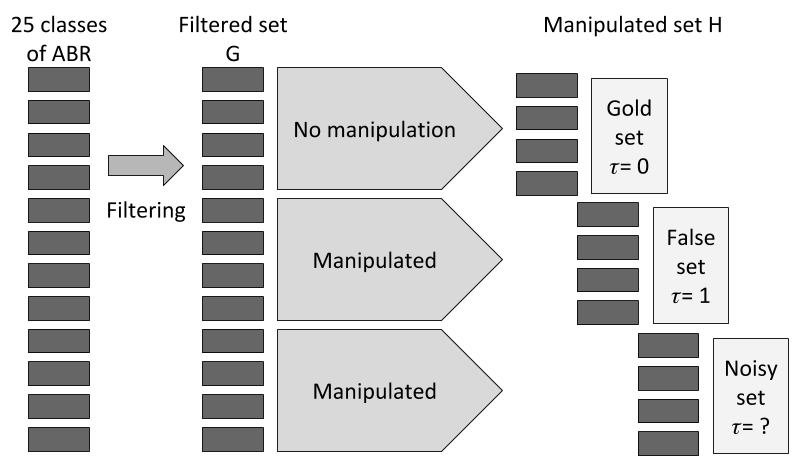
\includegraphics[width=\linewidth]{Synthethic set2}
\caption{Obtaining set $G$ and set $H$.}
\label{fig1}
\end{figure}

					%%%%%%%%%%
					\subsection{Experimental settings}
					\label{section:settings}
					%%%%%%%%%%
% representativity error-pattern
% size labeled set
% percentage of errors
% error type

% design model (with/without log reg)

We aim to test the performance of the algorithm in different settings. The manipulations in set $H$ are varied with respect to: 1) how representative the error-patterns in the labeled set is for the error-pattern in the noisy set, 2) the size of the labeled set compared to the noisy set, 3) the percentage of errors in the noisy set, and 4) the type of errors. 

Firstly, the error patterns in the labeled and noisy set could be generated such that they are similar, i.e. cases with certain characteristics have errors. This is referred to as the 'informed labeled set'. In this case, the model should be able to point out the errors in the noisy that. We also generate errors in the labeled set using only part of the enterprise characteristics, the 'limited labeled set'. Also, we can introduce random errors in the labeled set: 'random labeled set'. 

Two types of errors can be introduced: obvious and subtle errors. When a observed SBI code is manipulated, one could vary how related the new, manipulated label is to the observed label. A SBI code that is changed to a non-related SBI code is an obvious error. A SBI code that is changed to a more similar, related SBI code is a subtle error.

Moreover, the proposed model, including a machine learning model and a logistic regression model, can be simplified. Less predictors can be used in the logistic regression, or the logistic regression could be replaced by simply including an average error probability.

% Settings for the number of activitites;
% A machine learning model provides us with a probability for every class. So far, in the discussion of the algorithm, only the first predicted class (top 1) is considered. Instead, also the three most likely classes can be considered (top 3). We want to account for the fact that an enterprise can have multiple activities and a website may be biased towards a related activity.

Table \ref{tab:table2} gives an overview of the experimental settings. 

\begin{table}[h]
\caption{\label{tab:table2}Experimental settings.}
\centering 
\begin{tabular}{ll}
\hline
\textbf{Dataset}               &                                                                                                                                                                                                 \\ \hline
Representativity error-pattern & \begin{tabular}[c]{@{}l@{}}informed labeled set, \\ limited labeled set,\\ random labeled set\end{tabular}                                                                                      \\
Size labeled set               & ?\%, ?\%, ?\%                                                                                                                                                                                   \\
Percentage of errors           & 5\%, 10\%, 20\%                                                                                                                                                                                 \\
Error type                     & obvious, subtle                                                                                                                                                                                 \\ \hline
\textbf{Model}                 &                                                                                                                                                                                                 \\ \hline
Modeling $\pi_i$               & \begin{tabular}[c]{@{}l@{}}logistic regression to estimate $\pi_i$,\\ logistic regression (limited predictors) to estimate $\pi_i$,\\ use a fixed, average error probability $\pi$\end{tabular}
\end{tabular}
\end{table}




					%%%%%%%%%%
					\subsection{Evaluation metrics}
					\label{section:evaluation}
					%%%%%%%%%%


% verschillende startwaarden: log likelihood
\subsubsection{Log-likelihood}
In order to select the optimal starting values for the EM algorithm, we use the log-likelihood of the labeled set. Within the labeled set, there is a part with $z_i = 1$ and a part with $z_i = 0$. For the part with $z_i = 1$ we are interested in the estimated probabilities for $\tau_i$. These probabilities are ideally close to 1. For the part of the labeled set where $z_i = 0$, we do know the true SBI code for unit $i$. We want to extract the probability of for that code as predicted by the machine learning model. Preferably, this probability is close to 1.
The log-likelihood is then given by:

						\begin{equation}\label{log}
log \sum_i (z_i \tau_i + \sum_k (1-z_i)I(y_i = k)\hat{P}(y_i=k)
						\end{equation}

% Evaluate which of the SBI codes are predicted to be erroneous
\subsubsection{Cross-entropy loss}
The cross-entropy loss, also called log loss, is used to measure the performance of the different models considered in the experiments. The log loss is defined on probability estimates and, therefore, takes the uncertainty of the predicted labels into account. The further the value of the log loss deviates from 0, the further away the predicted probability is from the actual class. The log loss can be computed for binary classification problems with the \texttt{log\_loss} function in the \texttt{scikit-learn} package \citep{sklearn}. 


\bigskip

Next, the results of the experiments are discussed. After that, the model is applied to real data and the outcomes are discussed.


\clearpage % to make sure references are on separate page

\bibliographystyle{apacite} 
\bibliography{references_VO}

\end{document}

